\section{Concave upper bound of sofa area}

In this section, we show that the corner injectivity theorem \ref{thm:injective} provides us an upper bound $\cA_1(S)$ of the area $\cA(S)$ of a monotone sofa $S$ which is concave respect to $\xx$.
Assume in the following that the upper part of the cap $\cC(S)$ of monotone sofa $S$ is strictly convex and smooth.

% I'm following the derivation/notation provided by Yoav in a previous email.
% Then I will argue that the area of a monotone sofa is negative definite.

For any $t \in \RR$, define $u_t$ as the unit vector that makes an angle of $t$ from the $x$-axis.
And define $v_t = u_{t + \pi / 2}$ as the unit vector perpendicular to $u_t$.
We will use the wedge product $\vv_1 \times \vv_2 \in \RR$ of two vectors $\vv_1, \vv_2$ in $\RR^2$ which is defined as $(x_1, y_1) \times (x_2, y_2) = x_1 y_2 - x_2 y_1$.
For any $0 \leq t \leq \pi$, let $h(t)$ be the height function of the cap, and $A(t)$ be the corresponding point on the tangency.
That is, $h(t) = \max_{p \in \cC(S)} p \cdot u_t$
and $A(t) = \arg \max_{p \in \cC(S)} p \cdot u_t$.
Then we have $A(t) = h(t) u_t + h'(t) v_t$.
The area of the cap is $\frac{1}{2} \int_0^{\pi} A(t) \times A'(t) dt$, which simplifies to 
$\frac{1}{2} \int_0^{\pi} h(t)^2 + h(t)h''(t) dt$ using the equation above and $u_t \times v_t = -v_t \times u_t = 1$. 
For $0 \leq t \leq \pi / 2$, define $g(t) = h(t + \pi / 2)$.

Now we have a look at the area of the niche. 
By the injectivity theorem \ref{thm:injective}, it is possible to bound the area of the niche from below by the area determined by the inner corner $\xx$.
The inner corner's position is then $\xx(t) = (h(t) - 1) u_t + (g(t) - 1) v_t$.
The area of the niche would then be bounded from below by 
$\frac{1}{2} \int_0^{\pi / 2} \xx(t) \times \xx'(t)$. 
Keeping only the homogeneous quadratic terms, this is equal to
$\frac{1}{2} \int_0^{\pi / 2} h(t)^2+g(t)^2+h(t)g'(t)-g(t)h'(t) dt$.
Finally, subtracting the area of cap by the lower bound of the niche, the upper bound of sofa area determined by the path of inner corner $\xx$ is equal to
\begin{equation}
\label{eq:areaub}
\cA_1(S) = \frac{1}{2}\int_0^{\pi/2} h(t)h''(t)+g(t)g''(t)-h(t)g'(t)+g(t)h'(t) dt
\end{equation}
modulo linear terms respect to $h$ and $g$. This derivation so far is from Yoav's email. 

Let $B(t) = A(t + \pi / 2)$. Let $\yy(t)$ be the coordinate of the outer corner, so that $\yy(t) = h(t) u_t + g(t)v_t$. Then consequently we have
$B(t) = - g'(t) u_t + g(t)v_t $.
I claim that the area \eqref{eq:areaub} is equal to
\begin{equation}
\label{eq:areaquad}
\cA_1(S) = - \frac{1}{2} \int_0^{\pi / 2} 
\left(
\left((y(t) - B(t)) \cdot u_t \right)^2 + 
\left(\frac{1 - A(t) \cdot v_0}{\cos t} \right)^2 
\right) dt
\end{equation}
modulo linear terms.
It is the area of the region shaded blue in the following figure.
\begin{figure}%                 use [hb] only if necceccary!
  \centering
  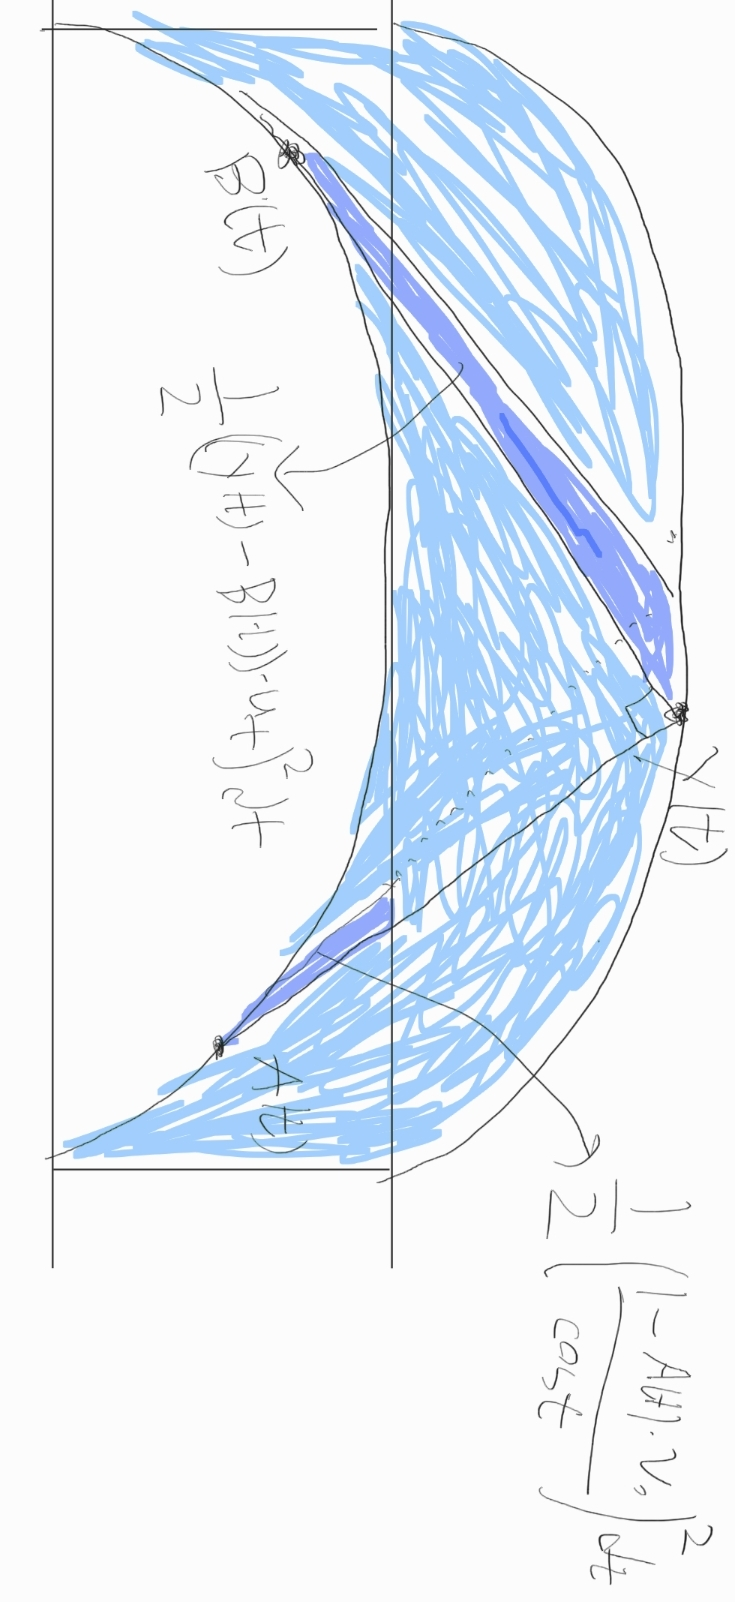
\includegraphics[width=10cm]{sofa.jpeg}
  \label{fig:test}
\end{figure}
One needs to use $h(\pi / 2) = 1$ to show this.
The integral form shows that $\cA_1$ is concave, which makes it subject to convex optimization.
